\section{Reducción de dimensiones}\label{sec:dimensionalityReduction}

\begin{frame}
    \frametitle{Análisis de Componentes Principales}

    \begin{columns}
        \pause
        \column{0.5\textwidth}

        \begin{block}{Covarianza}
            Medida de la dependencia lineal entre dos variables aleatorias $x,y\in \mathbb{R}^n$.

            \begin{equation*}
                \sigma_{x,y} = \frac{1}{n}\sum_{i=1}^{n}{(x_i - \bar{x})(y_i - \bar{y})}
            \end{equation*}
        \end{block}

        \pause
        \column{0.5\textwidth}

        Matriz de covarianza:
        \begin{equation*}
            \Sigma_X = \begin{bmatrix}
                           \sigma_{1,1} & \sigma_{1,2} & \ldots & \sigma_{1,m} \\
                           \sigma_{2,1} & \sigma_{2,2} & \ldots & \sigma_{2,m} \\
                           \vdots & \vdots & \ldots & \vdots \\
                           \sigma_{m,1} & \sigma_{m,2} & \ldots & \sigma_{m,m}
            \end{bmatrix}
        \end{equation*}

    \end{columns}
\end{frame}

\begin{frame}
    \frametitle{Análisis de Componentes Principales}

    \begin{block}{Transformar el espacio de los datos a uno donde las componentes sean linealmente independientes entre sí.}
        \begin{itemize}
            \item<2-> Cada par de atributos diferentes tiene covarianza 0.
            \item<3-> Los atributos se encuentran ordenados respecto a la cantidad de varianza de los datos.
        \end{itemize}
    \end{block}

    \begin{itemize}
        \item<4-> $\lambda_1 \geq \lambda_2 \geq \dots \geq \lambda_{m-1} \geq \lambda_{m} \geq 0$ valores propios de $\Sigma_X$.
        \item<5-> $U = [u_1,\dots,u_m]$ matriz donde cada columna $u_j$ es el vector propio de $\Sigma_X$ que corresponde al valor propio $\lambda_j$.
    \end{itemize}
\end{frame}

\begin{frame}
    \frametitle{Análisis de Componentes Principales}

    \begin{block}{Si la media de la matriz $X$ correspondiente al conjunto de datos es 0 se cumple que:}
        \begin{itemize}
            \item<2-> $\hat{X} = XU$ es la matriz correspondiente al conjunto de datos transformado, que cumple las condiciones mencionadas anteriormente.
            \item<3-> Cada nuevo atributo es una combinación lineal de los atributos originales.
            \item<4-> La varianza del $j$-ésimo atributo es $\lambda_j$.
            \item<5-> La suma de las varianzas de los atributos originales es igual a la suma de las varianzas de los nuevos atributos.
        \end{itemize}
    \end{block}
\end{frame}

\begin{frame}
    \frametitle{Análisis de Componentes Principales}

    \begin{figure}[!h]
        \centering
        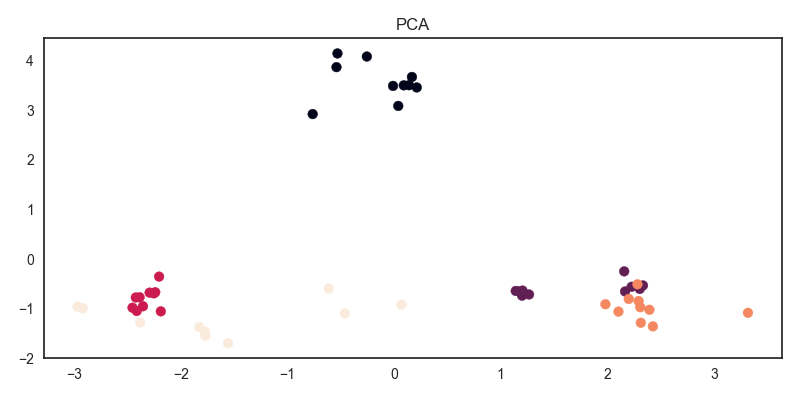
\includegraphics[width=\textwidth]{pca.png}
    \end{figure}

    {\footnotesize
    Resultado de aplicar PCA para reducir a dos las dimensiones de los MFCC de un conjunto de sonidos de cinco especies animales.
    }
\end{frame}


\begin{frame}
    \frametitle{Manifold Learning}

    \begin{columns}
        \column{0.5\textwidth}

        \begin{itemize}
            \item<2-> \textbf{Multi-dimensional Scaling (MDS)}
            \begin{equation*}
                \sum_{i=1}^{N}\sum_{j=i+1}^{N}{d_{ij} - \hat{d}_{ij}}
            \end{equation*}
            \item<3-> \textbf{Isomap} \\
            MDS sobre la \textit{distancia geodésica}
            \item<4-> \textbf{Locally Linear Embedding (LLE)}
        \end{itemize}

        \column{0.5\textwidth}

        \begin{figure}[!h]
            \centering
            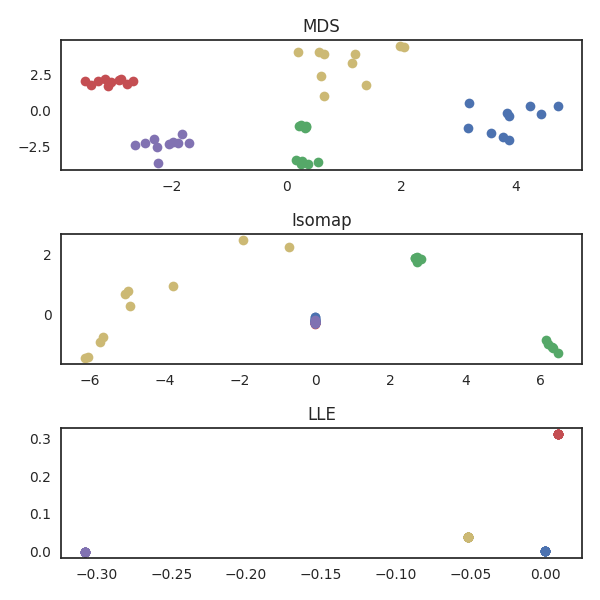
\includegraphics[width=\textwidth]{manifold-learning-vertical.png}
        \end{figure}

    \end{columns}
\end{frame}